%%%%%%%%%%%%%%%%%%%%%%%%%%%%%%%%%%%%%%%%%
% Short Sectioned Assignment LaTeX Template Version 1.0 (5/5/12)
% This template has been downloaded from: http://www.LaTeXTemplates.com
% Original author:  Frits Wenneker (http://www.howtotex.com)
% License: CC BY-NC-SA 3.0 (http://creativecommons.org/licenses/by-nc-sa/3.0/)
%%%%%%%%%%%%%%%%%%%%%%%%%%%%%%%%%%%%%%%%%

%----------------------------------------------------------------------------------------
%	PACKAGES AND OTHER DOCUMENT CONFIGURATIONS
%----------------------------------------------------------------------------------------

\documentclass[paper=a4, fontsize=11pt]{scrartcl} % A4 paper and 11pt font size

% ---- Entrada y salida de texto -----

\usepackage{hyperref}
\usepackage{listings}
\usepackage{color}
%AÑADIDO DE LA PÁGINA http://stackoverflow.com/questions/3175105/how-to-insert-code-into-a-latex-doc
\definecolor{dkgreen}{rgb}{0,0.6,0}
\definecolor{gray}{rgb}{0.5,0.5,0.5}
\definecolor{mauve}{rgb}{0.58,0,0.82}

\lstset{frame=tb,
	language=Python,
	aboveskip=3mm,
	belowskip=3mm,
	showstringspaces=false,
	columns=flexible,
	basicstyle={\small\ttfamily},
	numbers=none,
	numberstyle=\tiny\color{gray},
	keywordstyle=\color{blue},
	commentstyle=\color{dkgreen},
	stringstyle=\color{mauve},
	breaklines=true,
	breakatwhitespace=true,
	tabsize=3
}
%%%%%%%%%%%%%%%%%%%%%%%%%%%%%%%%%%%%%%%%%%%%%%%%%%%%%%%
\usepackage{varioref}
\usepackage[T1]{fontenc} % Use 8-bit encoding that has 256 glyphs
\usepackage[utf8]{inputenc}
%\usepackage{fourier} % Use the Adobe Utopia font for the document - comment this line to return to the LaTeX default

% ---- Idioma --------

\usepackage[spanish, es-tabla]{babel} % Selecciona el español para palabras introducidas automáticamente, p.ej. "septiembre" en la fecha y especifica que se use la palabra Tabla en vez de Cuadro

% ---- Otros paquetes ----

\usepackage{amsmath,amsfonts,amsthm} % Math packages
%\usepackage{graphics,graphicx, floatrow} %para incluir imágenes y notas en las imágenes
\usepackage{graphics,graphicx, float} %para incluir imágenes y colocarlas

% Para hacer tablas comlejas
%\usepackage{multirow}
%\usepackage{threeparttable}

%\usepackage{sectsty} % Allows customizing section commands
%\allsectionsfont{\centering \normalfont\scshape} % Make all sections centered, the default font and small caps

\usepackage{fancyhdr} % Custom headers and footers
\pagestyle{fancyplain} % Makes all pages in the document conform to the custom headers and footers
\fancyhead{} % No page header - if you want one, create it in the same way as the footers below
\fancyfoot[L]{} % Empty left footer
\fancyfoot[C]{} % Empty center footer
\fancyfoot[R]{\thepage} % Page numbering for right footer
\renewcommand{\headrulewidth}{0pt} % Remove header underlines
\renewcommand{\footrulewidth}{0pt} % Remove footer underlines
\setlength{\headheight}{13.6pt} % Customize the height of the header

\numberwithin{equation}{section} % Number equations within sections (i.e. 1.1, 1.2, 2.1, 2.2 instead of 1, 2, 3, 4)
\numberwithin{figure}{section} % Number figures within sections (i.e. 1.1, 1.2, 2.1, 2.2 instead of 1, 2, 3, 4)
\numberwithin{table}{section} % Number tables within sections (i.e. 1.1, 1.2, 2.1, 2.2 instead of 1, 2, 3, 4)

\setlength\parindent{0pt} % Removes all indentation from paragraphs - comment this line for an assignment with lots of text

\newcommand{\horrule}[1]{\rule{\linewidth}{#1}} % Create horizontal rule command with 1 argument of height


\renewcommand{\reftextbefore}
	{en la  \reftextvario{página que precede a esta}{página anterior}}
\renewcommand{\reftextafter}
	{en la \reftextvario{siguiente}{siguiente} página}
\renewcommand{\reftextfacebefore}
	{en la  \reftextvario{anterior}{anterior} página}
\renewcommand{\reftextfaceafter}
	{en la \reftextvario{siguiente}{siguiente}{página}}

 \usepackage{algpseudocode}
%----------------------------------------------------------------------------------------
%	TÍTULO Y DATOS DEL ALUMNO
%----------------------------------------------------------------------------------------

\title{	
\normalfont \normalsize 
\textsc{{\bf Algorítmica (2015-2016)} \\ Grado en Ingeniería Informática \\ Universidad de Granada} \\ [25pt] % Your university, school and/or department name(s)
\horrule{0.5pt} \\[0.4cm] % Thin top horizontal rule
\huge Práctica 1: Análisis de eficiencia de algoritmos \\ % The assignment title
\horrule{2pt} \\[0.5cm] % Thick bottom horizontal rule
}

\author{Francisco Carrillo Pérez,Borja Cañavate Bordons, \\Miguel Porcel Jiménez,Jose Manuel Rejón Santiago,Jose Arcos Aneas} % Nombre y apellidos

\date{\normalsize\today} % Incluye la fecha actual

%----------------------------------------------------------------------------------------
% DOCUMENTO
%----------------------------------------------------------------------------------------

\begin{document}

\maketitle % Muestra el Título

\newpage %inserta un salto de página

\tableofcontents % para generar el índice de contenidos

\listoffigures

\listoftables

\newpage

\section{Introducción }

El objetivo de ésta práctica es analizar implementar y comparar una solución divide y vencerás.
Para ello, hemos recogido los diferentes tiempos de los diferentes algoritmos que hemos diseñado y los hemos comparado.
En nuestro caso concreto, hemos utilizado la biblioteca de C++ más moderna y precisa destinado a obtener tiempos de reloj: la biblioteca \textbf{chrono}

La máquina que hemos utilizado tiene las siguientes características:
	
\begin{itemize}
		
	\item Procesador: Intel Core i5-3337U (2.7GHz x 2)
	\item Memoria RAM: 4GB
	\item Disco Duro: 500GB 5400 rpm
	\item SO: Manjaro Linux 15.2 Capella 64 bits
\end{itemize}
	



%------------------------------------------------
\section{Fuerza bruta} % Sections can be created in order to organize your presentation into discrete blocks, all sections and subsections are automatically printed in the table of contents as an overview of the talk
%------------------------------------------------

En esta sección hemos diseñado un algoritmo de fuerza bruta cuyo funcionamiento es el siguiente:

	\begin{algorithmic}
		\Require Vectores ordenados, numero de estos y tamaño
		
		\State{V1 = V[0]}
		\State{Vfinal = V[1]}
		\State{Vfinal = OrdenarVectores(V1,Vfinal)}
		\For {i=2 hasta i=k-1 }
		\State{V1=V[i]; }
		\State{Vfinal= OrdenarVectores(V1,Vfinal);}
		\State{i++;}
		\EndFor
	\end{algorithmic}


	\begin{figure}[H]
\centering
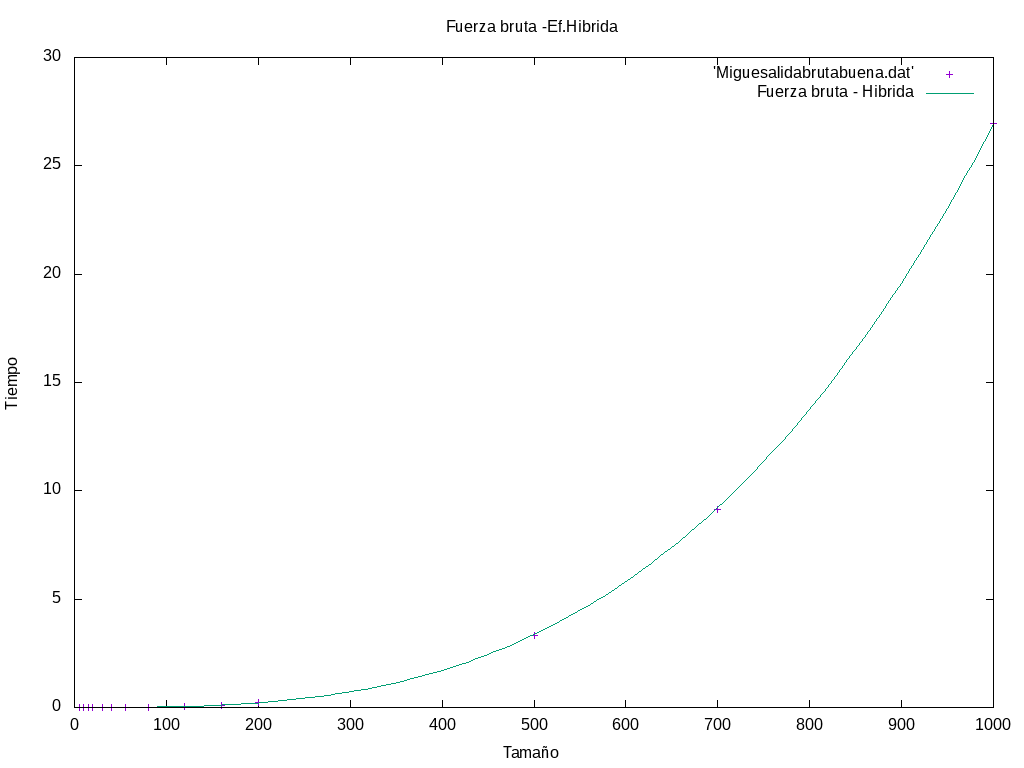
\includegraphics[width=0.7\linewidth]{../salidas-algoritmos/fuerzabruta-hibrida}
\caption{}
\label{fig:fuerzabruta-hibrida}
\end{figure}



\section{Algoritmo DyV} % Sections can be crea es muy bajoted in order to organize your presentation into discrete blocks, all sections and subsections are automatically printed in the table of contents as an overview of the talk
%------------------------------------------------
 La estructura y el funcionamiento de nuestro código es el siguiente:
 
 \textbf{Recursivo(matriz)}
 \begin{algorithmic}	
 	\Require Matriz de vectores
 	\If{ Si el número de vectores menor o igual a 1}	
 	
 	\Return La matriz con una fila
 	\Else{ Si el número de vectores es mayor que 1 }		 
 	\State{middle=nº filas/2 }
 	\State{Up = matriz[:middle][num\_colum]}
 	\State{Down = matriz[middle:][num\_colum]}
 	\State{Up = Recursivo(Up)}
 	\State{Down = Recursivo(Down)}		 
 	\State{Result = Merge(Up, Down) }
 	
 	\Return Result
 	\EndIf
 	
 \end{algorithmic}	
 
 	La eficiencia obtenida ha resultado ser de \textbf{n2} ,mejorando en un orden al de fuerza bruta.
 	\begin{figure}[H]
 		\centering
 		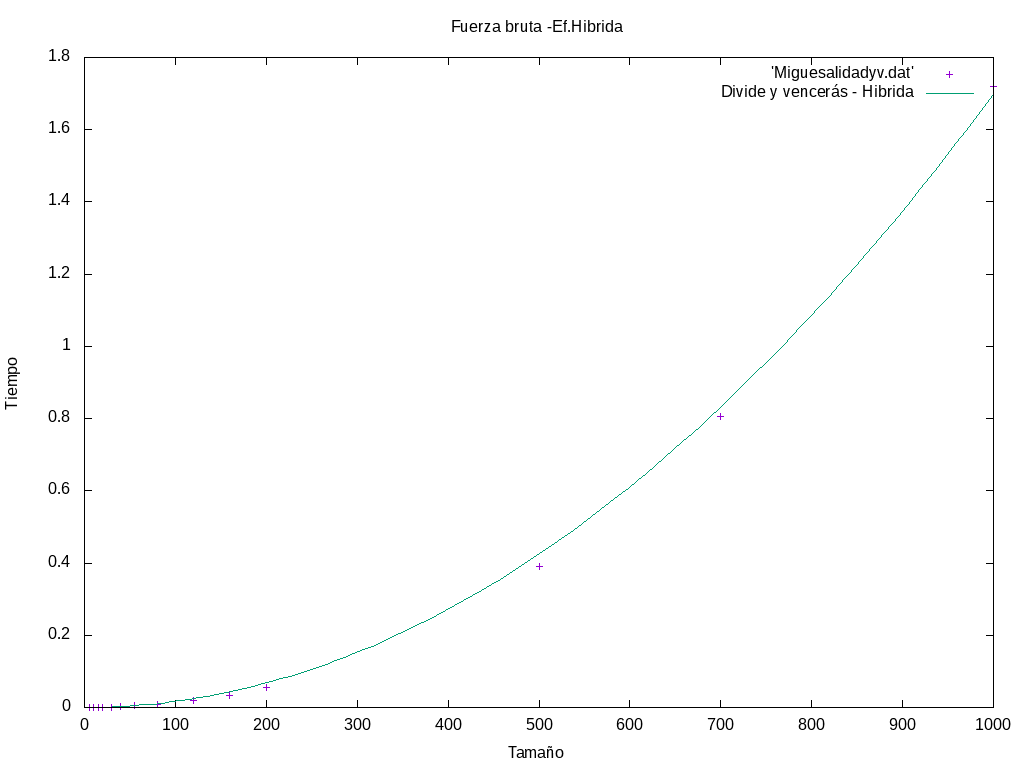
\includegraphics[width=0.7\linewidth]{../salidas-algoritmos/dyv-hibrida.png}
 		\caption{Figura perteneciente a la eficiencia híbrida obtenida}
 		\label{fig:fuerzabruta-hibrida}
 	\end{figure}
 	
 \section{Comparación} % Sections can be created in order to organize your presentation into discrete blocks, all sections and subsections are automatically printed in the table of contents as an overview of the talk
 %------------------------------------------------
 	En esta última sección, hemos comparado los dos algoritmos que hemos desarrollado, veremos si efectivamente o no nuestra implementación utilizando un enfoque divide y vencerás obtenemos mejoras con respecto a uno de fuerza bruta.
 	
 

 	\begin{figure}[H]
 		\centering
 		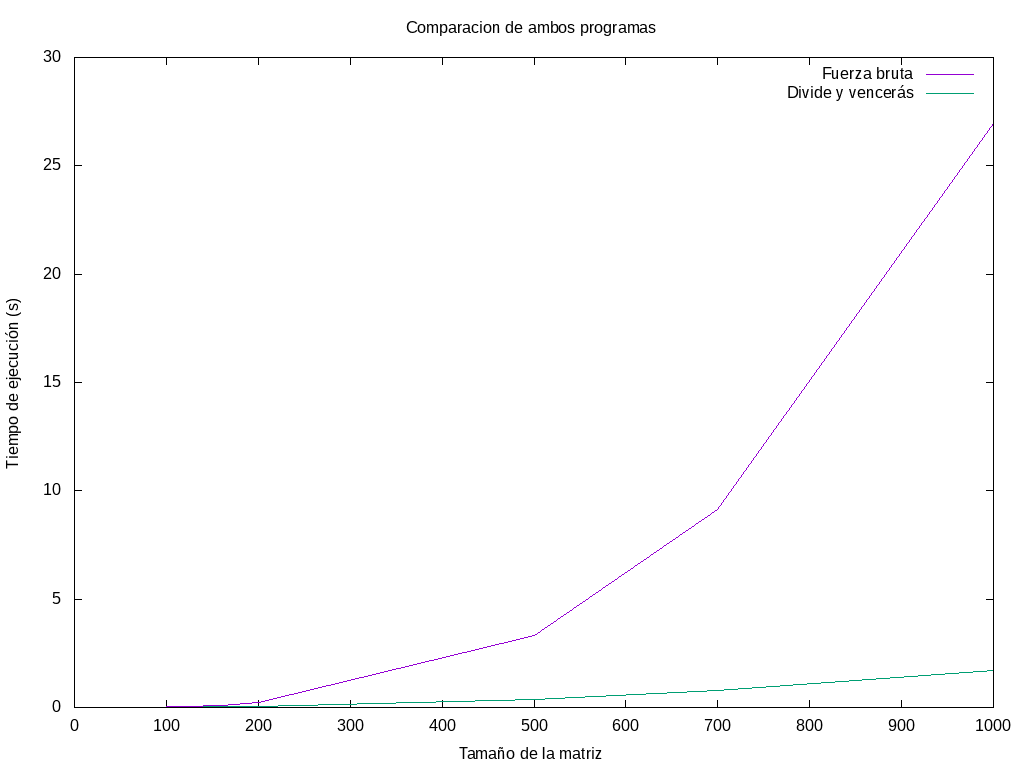
\includegraphics[width=0.7\linewidth]{../salidas-algoritmos/comparacion.png}
 		\caption{Figura perteneciente a la comparación entre ambas eficiencias}
 		\label{fig:fuerzabruta-hibrida}
 	\end{figure}

\section{Porcentaje de error y constantes ocultas}
Por último, mostramos el porcentaje de error así como las constantes ocultas.\\
\begin{center}
	\begin{tabular}{| l | c | r |}
		\hline
		\textbf{Algoritmo} & \textbf{Constante Oculta} & \textbf{Error} \\ \hline
		DyV & a0 = 1.69804e-06  & +/- 1.226e-08    (0.7218\%)\\ 
		\hline
		Fuerza bruta & a0 = 2.69052e-08 & +/- 2.352e-11    (0.0874\%)
		
	\end{tabular}
\end{center}


%----------------------------------------------------------------------------------------

\end{document}